\chapter{Resultados e Discussões}

A ferramenta proposta gerou o dataset multimodal composto de dados de EEG e ET a partir de código 
de coleta construído com MATLAB e limpeza de dados por Python. A ferramenta utiliza a capacidade do 
equipamento GP3 de receber informações definidas pelo usuário, para capturar informação sobre a onda de EEG advinda 
do atributo raw do produto Mindwave Mobile II. 

\begin{figure}[!h]
    \centering
    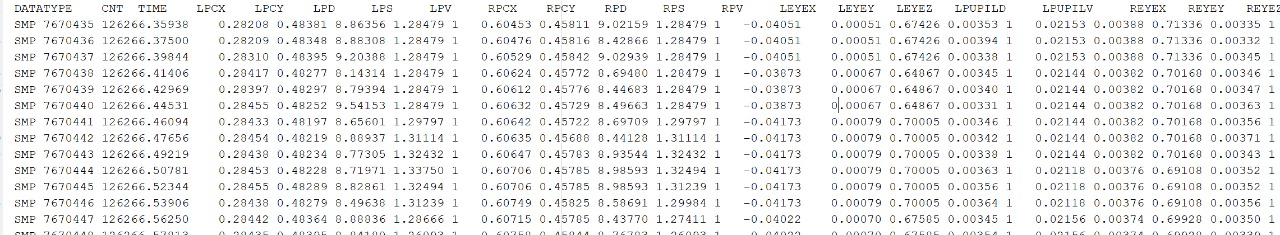
\includegraphics[width=160mm]{example_dataset.jpeg}
    \caption{Exemplo de arquivo TXT depois de coleta.}
\end{figure}

\section{Características da Ferramenta}
Como a ferramenta utiliza a opção de envio de código do USER (GP3) para captura dos dados de EEG, 
o dataset ja é composto da junção por \textit{feature level} de EEG e ET, com a mesma frequência amostral. 

\begin{figure}[!h]
    \centering
    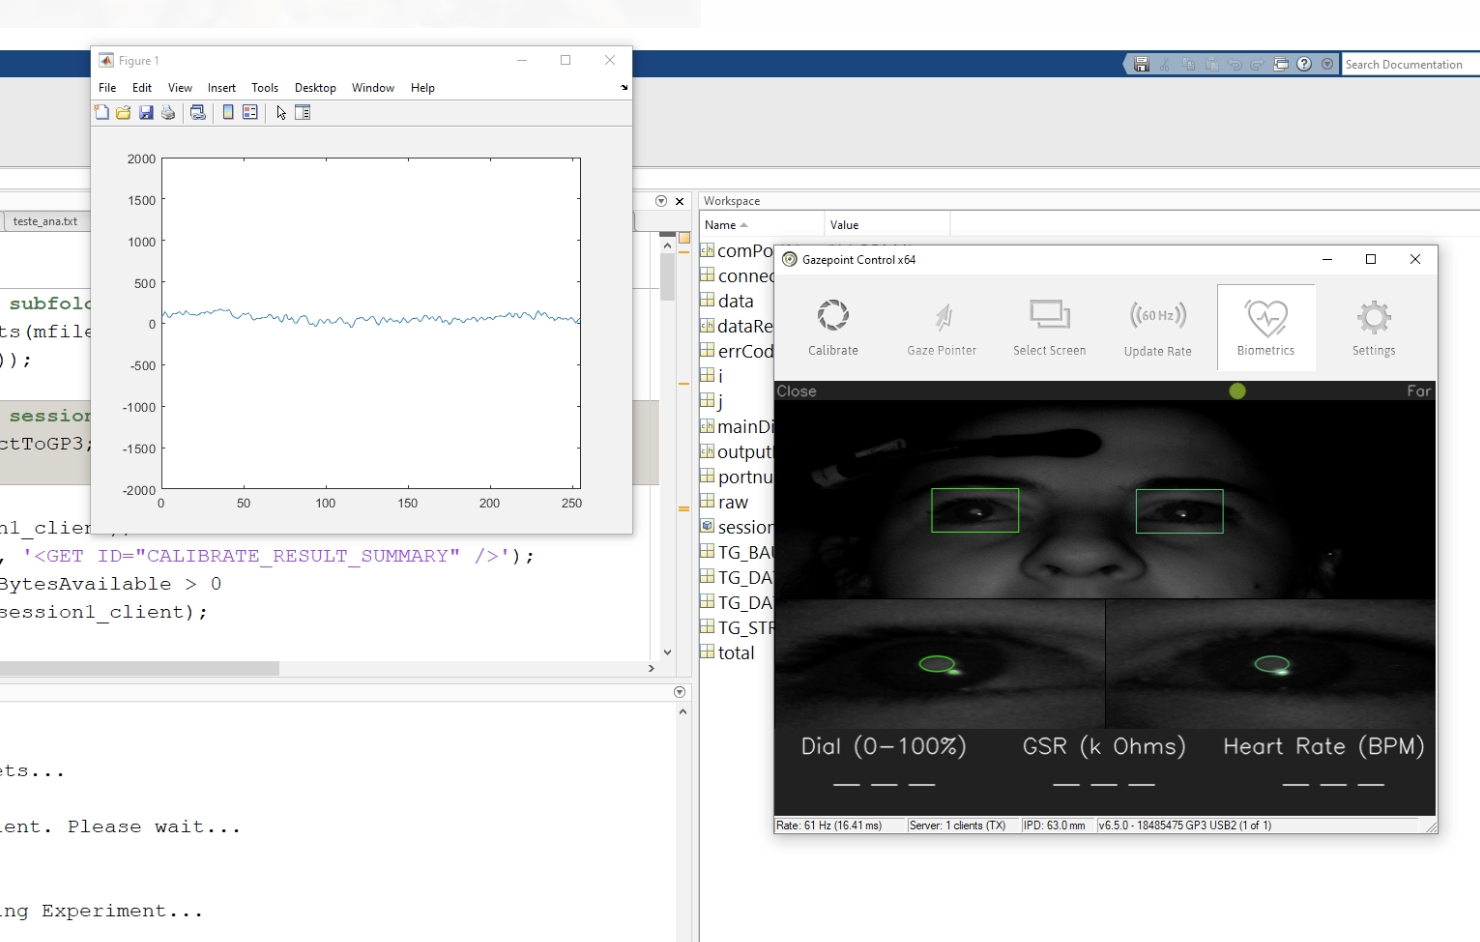
\includegraphics[width=200mm]{real-time-plot-and-et.png}
    \caption{Janela com o plot em tempo real da coleta de EEG e identificação de piscadas.}
\end{figure}

\clearpage

\section{Usabilidade: Resultados do Estudo de Caso}
O primeiro estudo de caso levantado para a ferramenta consistiu na análise do poder classificatório de algortimos 
treinados com o dataset resultante da ferramenta. 

subsection{Atividade: Apresentação de Estímulo Visual Negativo e Positivo}

\section{Discussão}